I test sono stati effettuati su un dataset da 1000 fino a 10000000 email, con una probabilità di falsi positivi di
0.10, 0.05 e 0.01.

\subsection{FPR: 0.05}\label{subsec:fpr-005}
\subsubsection{Setup}\label{subsubsec:fpr-005-setup}
\begin{figure}[H]
    \centering
    \minipage{0.49\textwidth}
    \includegraphics[width=\linewidth]{openmp/005/setup_times}
        \caption{Time setup Omp}\label{fig:005-setup_time_omp}
    \endminipage\hfill
    \minipage{0.49\textwidth}
    \includegraphics[width=\linewidth]{joblib/005/setup_time_plot}
        \caption{Time setup Joblib}\label{fig:005-setup_time_joblib}
    \endminipage\hfill
\end{figure}
\begin{figure}[H]
    \centering
    \minipage{0.49\textwidth}
    \includegraphics[width=\linewidth]{openmp/005/setup_speedup}
        \caption{Speedup setup Omp}\label{fig:005-setup_speedup_omp}
    \endminipage\hfill
    \minipage{0.49\textwidth}
    \includegraphics[width=\linewidth]{joblib/005/setup_speedup_plot}
        \caption{Speedup setup Joblib}\label{fig:005-setup_speedup_joblib}
    \endminipage\hfill
\end{figure}
\begin{figure}[H]
    \centering
    \minipage{0.49\textwidth}
    \includegraphics[width=\linewidth]{openmp/005/setup_fpr}
        \caption{FPR setup Omp}\label{fig:005-setup_fpr_omp}
    \endminipage\hfill
    \minipage{0.49\textwidth}
    \includegraphics[width=\linewidth]{joblib/005/setup_fpr_plot}
        \caption{FPR setup Joblib}\label{fig:005-setup_fpr_joblib}
    \endminipage\hfill
\end{figure}

Per il test di configurazione iniziale, è evidente che la versione sviluppata con OpenMP presenta una performance
temporale inferiore rispetto alla controparte.
Al contrario, in termini di speedup, la versione OpenMP supera la versione sviluppata con Joblib,
raggiungendo uno speedup massimo di 2.70 nella versione Joblib e 9 nella versione OpenMP, utilizzando il massimo
numero di thread disponibili.

I risultati massimi sono stati ottenuti sfruttando il numero massimo di thread disponibili.
Nel contesto della versione Joblib, i test iniziali con un numero più elevato di thread mostrano un tempo di esecuzione
peggiore rispetto alla versione sequenziale, probabilmente a causa del tempo di inizializzazione dei thread.
Nonostante l'aumento del numero di thread nella versione Joblib, lo speedup si stabilizza intorno al valore di 2.

Va notato che i valori di FPR (False Positive Rate) sono molto simili tra le due versioni.

\subsubsection{Filter}\label{subsubsec:fpr-005-filter}
\begin{figure}[H]
    \centering
    \minipage{0.49\textwidth}
    \includegraphics[width=\linewidth]{openmp/005/filter1_times}
        \caption{Time Filter Omp}\label{fig:005-filter_time_omp}
    \endminipage\hfill
    \minipage{0.49\textwidth}
    \includegraphics[width=\linewidth]{joblib/005/filter_time_plot}
        \caption{Time Filter Joblib}\label{fig:005-filter_time_joblib}
    \endminipage\hfill
\end{figure}
\begin{figure}[H]
    \centering
    \minipage{0.49\textwidth}
    \includegraphics[width=\linewidth]{openmp/005/filter1_speedup}
        \caption{Speedup Filter Omp}\label{fig:005-filter_speedup_omp}
    \endminipage\hfill
    \minipage{0.49\textwidth}
    \includegraphics[width=\linewidth]{joblib/005/filter_speedup_plot}
        \caption{Speedup Filter Joblib}\label{fig:005-filter_speedup_joblib}
    \endminipage\hfill
\end{figure}
\begin{figure}[H]
    \centering
    \minipage{0.49\textwidth}
    \includegraphics[width=\linewidth]{openmp/005/filter_fpr}
        \caption{FPR Filter Omp}\label{fig:005-filter_fpr_omp}
    \endminipage\hfill
    \minipage{0.49\textwidth}
    \includegraphics[width=\linewidth]{joblib/005/filter_fpr_plot}
        \caption{FPR Filter Joblib}\label{fig:005-filter_fpr_joblib}
    \endminipage\hfill
\end{figure}

Per il test di filtraggio, è evidente che la versione sviluppata con OpenMP presenta una performance temporale
inferiore rispetto alla sua controparte.
Tuttavia, in termini di speedup, la versione OpenMP supera la versione sviluppata con Joblib, raggiungendo un
massimo di 11 nella versione OpenMP e 2.5 nella versione Joblib, sfruttando il massimo numero di thread disponibili.

Anche in questo contesto, i valori di FPR (False Positive Rate) sono praticamente identici tra le due versioni.

\subsubsection{Chunks}\label{subsubsec:005-chunks}
Esploriamo ora l'opzione di eseguire un'operazione di chunking più ampia rispetto al numero di thread disponibili per
verificare se è possibile migliorare le performance, focalizzandoci esclusivamente sulla versione Joblib.
I valori di riferimento per i chunks sono 16, 32, 64, 128, 256, 512, 1024, 2048.

\begin{figure}[H]
    \centering
    \minipage{0.49\textwidth}
    \includegraphics[width=\linewidth]{joblib/005/chunks_time_plot}
        \caption{Times setup Chunks}\label{fig:005-chunks_time}
    \endminipage\hfill
    \minipage{0.49\textwidth}
    \includegraphics[width=\linewidth]{joblib/005/chunks_speedup_plot}
        \caption{Speedup setup Chunks}\label{fig:005-chunks_speedup}
    \endminipage\hfill
\end{figure}

I risultati ottenuti indicano che l'applicazione dell'operazione di chunking ha determinato miglioramenti
significativi nelle performance di speedup.
In particolare, l'aumento del numero di chunk ha contribuito a un miglioramento dello speedup,
raggiungendo un massimo di 3.
Tuttavia, oltre una soglia di 64 chunk, si è verificato un declino nelle performance.

\subsection{FPR: 0.01}\label{subsec:fpr-001}
Vediamo adesso se aumentando la precisione del filtro, i risultati ottenuti precedentemente cambiano.

\subsubsection{Setup}\label{subsubsec:setup}
\begin{figure}[H]
    \centering
    \minipage{0.49\textwidth}
    \includegraphics[width=\linewidth]{openmp/001/setup_times}
        \caption{Speedup setup Omp}\label{fig:setup_time_omp}
    \endminipage\hfill
    \minipage{0.49\textwidth}
    \includegraphics[width=\linewidth]{joblib/001/setup_time_plot}
        \caption{Speedup setup Joblib}\label{fig:setup_time_joblib}
    \endminipage\hfill
\end{figure}
\begin{figure}[H]
    \centering
    \minipage{0.49\textwidth}
    \includegraphics[width=\linewidth]{openmp/001/setup_speedup}
        \caption{Speedup setup Omp}\label{fig:setup_speedup_omp}
    \endminipage\hfill
    \minipage{0.49\textwidth}
    \includegraphics[width=\linewidth]{joblib/001/setup_speedup_plot}
        \caption{Speedup setup Joblib}\label{fig:setup_speedup_joblib}
    \endminipage\hfill
\end{figure}
\begin{figure}[H]
    \centering
    \minipage{0.49\textwidth}
    \includegraphics[width=\linewidth]{openmp/001/setup_fpr}
        \caption{Speedup setup Omp}\label{fig:setup_fpr_omp}
    \endminipage\hfill
    \minipage{0.49\textwidth}
    \includegraphics[width=\linewidth]{joblib/001/setup_fpr_plot}
        \caption{Speedup setup Joblib}\label{fig:setup_fpr_joblib}
    \endminipage\hfill
\end{figure}

In questo contesto, nella fase di setup,
i risultati ottenuti indicano un aumento delle tempistiche di esecuzione per la versione Joblib
rispetto a FP=0.05, tuttavia si osserva un miglioramento in termini di speedup, che raggiunge un massimo di 3.1.
Al contrario, la versione OpenMP manifesta un peggioramento nelle performance di speedup,
raggiungendo un massimo di 7.1 con il massimo numero di thread disponibili.
Anche in questo caso, i valori di FPR (False Positive Rate) sono molto simili tra le due versioni, oscillando intorno
al valore di 0.01.

\subsubsection{Filter}\label{subsubsec:filter}
\begin{figure}[H]
    \centering
    \minipage{0.49\textwidth}
    \includegraphics[width=\linewidth]{openmp/001/filter1_times}
        \caption{Times filter Omp}\label{fig:filter_time_omp}
    \endminipage\hfill
    \minipage{0.49\textwidth}
    \includegraphics[width=\linewidth]{joblib/001/filter_time_plot}
        \caption{Times filter Joblib}\label{fig:filter_time_joblib}
    \endminipage\hfill
\end{figure}
\begin{figure}[H]
    \centering
    \minipage{0.49\textwidth}
    \includegraphics[width=\linewidth]{openmp/001/filter1_speedup}
        \caption{Speedup filter Omp}\label{fig:filter_speedup_omp}
    \endminipage\hfill
    \minipage{0.49\textwidth}
    \includegraphics[width=\linewidth]{joblib/001/filter_speedup_plot}
        \caption{Speedup filter Joblib}\label{fig:filter_speedup_joblib}
    \endminipage\hfill
\end{figure}
\begin{figure}[H]
    \centering
    \minipage{0.49\textwidth}
    \includegraphics[width=\linewidth]{openmp/001/filter_fpr}
        \caption{FPR filter Omp}\label{fig:filter_fpr_omp}
    \endminipage\hfill
    \minipage{0.49\textwidth}
    \includegraphics[width=\linewidth]{joblib/001/filter_fpr_plot}
        \caption{FPR filter Joblib}\label{fig:filter_fpr_joblib}
    \endminipage\hfill
\end{figure}

Con l'aumento della precisione del filtro, i risultati ottenuti indicano un leggero peggioramento delle performance,
dovuto al numero maggiore di operazioni da eseguire rispetto a FP=0.05.

\subsubsection{Chunks}\label{subsubsec:chunks}
\begin{figure}[H]
    \centering
    \minipage{0.49\textwidth}
    \includegraphics[width=\linewidth]{joblib/001/chunks_time_plot}
        \caption{Times chunks Joblib}\label{fig:chunks_time_joblib}
    \endminipage\hfill
    \minipage{0.49\textwidth}
    \includegraphics[width=\linewidth]{joblib/001/chunks_speedup_plot}
        \caption{Speedup chunks Joblib}\label{fig:chunks_speedup_joblib}
    \endminipage\hfill
\end{figure}

Nella fase di chunking, i risultati ottenuti mostrano un miglioramento delle performance di speedup, raggiungendo un
massimo di 3.3.
Il valore di soglia per il numero di chunk rimane 64, oltre il quale si verifica un declino nelle performance.

\subsection{FPR: 0.10}\label{subsec:fpr-010}
Viceversa vediamo se diminuendo la precisione del filtro, i risultati ottenuti cambiano.

\subsubsection{Setup}\label{subsubsec:fpr-010-setup}
\begin{figure}[H]
    \centering
    \minipage{0.49\textwidth}
    \includegraphics[width=\linewidth]{openmp/010/setup_times}
        \caption{Time setup Omp}\label{fig:010-setup_time_omp}
    \endminipage\hfill
    \minipage{0.49\textwidth}
    \includegraphics[width=\linewidth]{joblib/010/setup_time_plot}
        \caption{Time setup Joblib}\label{fig:010setup_time_joblib}
    \endminipage\hfill
\end{figure}
\begin{figure}[H]
    \centering
    \minipage{0.49\textwidth}
    \includegraphics[width=\linewidth]{openmp/010/setup_speedup}
        \caption{Speedup setup Omp}\label{fig:010-setup_speedup_omp}
    \endminipage\hfill
    \minipage{0.49\textwidth}
    \includegraphics[width=\linewidth]{joblib/010/setup_speedup_plot}
        \caption{Speedup setup Joblib}\label{fig:010-setup_speedup_joblib}
    \endminipage\hfill
\end{figure}
\begin{figure}[H]
    \centering
    \minipage{0.49\textwidth}
    \includegraphics[width=\linewidth]{openmp/010/setup_fpr}
        \caption{FPR setup Omp}\label{fig:010-setup_fpr_omp}
    \endminipage\hfill
    \minipage{0.49\textwidth}
    \includegraphics[width=\linewidth]{joblib/010/setup_fpr_plot}
        \caption{FPR setup Joblib}\label{fig:010-setup_fpr_joblib}
    \endminipage\hfill
\end{figure}

In termini di tempo nella fase di setup, i risultati ottenuti indicano un peggioramento delle performance per la
versione OpenMP, rispetto al valore di FPR=0.05.
La versione Joblib, invece, mostra un peggioramento nelle fasi iniziali del test per poi stabilizzarsi intorno al
valore di 2.5 per il massimo numero di thread disponibili.

\subsubsection{Filter}\label{subsubsec:fpr-010-filter}
\begin{figure}[H]
    \centering
    \minipage{0.49\textwidth}
    \includegraphics[width=\linewidth]{openmp/010/filter1_times}
        \caption{Time setup Omp}\label{fig:010-filter_time_omp}
    \endminipage\hfill
    \minipage{0.49\textwidth}
    \includegraphics[width=\linewidth]{joblib/010/filter_time_plot}
        \caption{Speedup setup Joblib}\label{fig:010-filter_time_joblib}
    \endminipage\hfill
\end{figure}
\begin{figure}[H]
    \centering
    \minipage{0.49\textwidth}
    \includegraphics[width=\linewidth]{openmp/010/filter1_speedup}
        \caption{Speedup setup Omp}\label{fig:010-filter_speedup_omp}
    \endminipage\hfill
    \minipage{0.49\textwidth}
    \includegraphics[width=\linewidth]{joblib/010/filter_speedup_plot}
        \caption{Speedup setup Joblib}\label{fig:010-filter_speedup_joblib}
    \endminipage\hfill
\end{figure}
\begin{figure}[H]
    \centering
    \minipage{0.49\textwidth}
    \includegraphics[width=\linewidth]{openmp/010/filter_fpr}
        \caption{FPR Filter Omp}\label{fig:010-filter_fpr_omp}
    \endminipage\hfill
    \minipage{0.49\textwidth}
    \includegraphics[width=\linewidth]{joblib/010/filter_fpr_plot}
        \caption{FPR Filter Joblib}\label{fig:010-filter_fpr_joblib}
    \endminipage\hfill
\end{figure}

Per la fase di filtraggio, i risultati risultano essere molto simili a quelli ottenuti con FPR=0.05.

\subsubsection{Chunks}\label{subsubsec:010-chunks}
\begin{figure}[H]
    \centering
    \minipage{0.49\textwidth}
    \includegraphics[width=\linewidth]{joblib/010/chunks_time_plot}
        \caption{Times setup Chunk}\label{fig:010-chunks_time}
    \endminipage\hfill
    \minipage{0.49\textwidth}
    \includegraphics[width=\linewidth]{joblib/010/chunks_speedup_plot}
        \caption{Speedup setup Chunk}\label{fig:010-chunks_speedup}
    \endminipage\hfill
\end{figure}

Nella fase di chunking, i risultati ottenuti mostrano come il valore di soglia di chunk sia 256, oltre il quale si
verifica un declino nelle performance.


